%% Преамбула TeX-файла

% 1. Стиль и язык
\documentclass[utf8x, times, 14pt]{G7-32} % Стиль (по умолчанию будет 14pt)

% Остальные стандартные настройки убраны в preamble.inc.tex.
\sloppy

% Настройки стиля ГОСТ 7-32
% Для начала определяем, хотим мы или нет, чтобы рисунки и таблицы нумеровались в пределах раздела, или нам нужна сквозная нумерация.
\EqInChapter % формулы будут нумероваться в пределах раздела
\TableInChapter % таблицы будут нумероваться в пределах раздела
\PicInChapter % рисунки будут нумероваться в пределах раздела

% Добавляем гипертекстовое оглавление в PDF
\usepackage[
bookmarks=true, colorlinks=true, unicode=true,
urlcolor=black,linkcolor=black, anchorcolor=black,
citecolor=black, menucolor=black, filecolor=black,
]{hyperref}
\usepackage{pgfplots}
\usepackage{nomencl}

\usepackage{float}

\AfterHyperrefFix

\usepackage{microtype}% полезный пакет для микротипографии, увы под xelatex мало чего умеет, но под pdflatex хорошо улучшает читаемость

% Тире могут быть невидимы в Adobe Reader
\ifInvisibleDashes
\MakeDashesBold
\fi

\usepackage{graphicx}   % Пакет для включения рисунков

% С такими оно полями оно работает по-умолчанию:
% \RequirePackage[left=20mm,right=10mm,top=20mm,bottom=20mm,headsep=0pt,includefoot]{geometry}
% Если вас тошнит от поля в 10мм --- увеличивайте до 20-ти, ну и про переплёт не забывайте:
\geometry{right=10mm}
\geometry{left=30mm}
\geometry{bottom=20mm}
\geometry{ignorefoot}% считать от нижней границы текста


% Пакет Tikz
\usepackage{tikz}
\usetikzlibrary{arrows,positioning,shadows}

% Произвольная нумерация списков.
\usepackage{enumerate}

% ячейки в несколько строчек
\usepackage{multirow}

% itemize внутри tabular
\usepackage{paralist,array}

%\setlength{\parskip}{1ex plus0.5ex minus0.5ex} % разрыв между абзацами
\setlength{\parskip}{1ex} % разрыв между абзацами
\usepackage{blindtext}

% Центрирование подписей к плавающим окружениям
%\usepackage[justification=centering]{caption}

\usepackage{newfloat}
\DeclareFloatingEnvironment[
placement={!ht},
name=Equation
]{eqndescNoIndent}
\edef\fixEqndesc{\noexpand\setlength{\noexpand\parindent}{\the\parindent}\noexpand\setlength{\noexpand\parskip}{\the\parskip}}
\newenvironment{eqndesc}[1][!ht]{%
    \begin{eqndescNoIndent}[#1]%
\fixEqndesc%
}
{\end{eqndescNoIndent}}

\usepackage{afterpage}

\newcommand\blankpage{
	\null
	\thispagestyle{empty}
	\newpage
}



% Настройки листингов.
\ifPDFTeX
% 8 Листинги

\usepackage{listings}

% Значения по умолчанию
\lstset{
  basicstyle= \footnotesize,
  breakatwhitespace=true,% разрыв строк только на whitespacce
  breaklines=true,       % переносить длинные строки
%   captionpos=b,          % подписи снизу -- вроде не надо
  inputencoding=koi8-r,
  numbers=left,          % нумерация слева
  numberstyle=\footnotesize,
  showspaces=false,      % показывать пробелы подчеркиваниями -- идиотизм 70-х годов
  showstringspaces=false,
  showtabs=false,        % и табы тоже
  stepnumber=1,
  tabsize=4,              % кому нужны табы по 8 символов?
  frame=single,
  xleftmargin=2.4em,
  framexleftmargin=2em
}

% Стиль для псевдокода: строчки обычно короткие, поэтому размер шрифта побольше
\lstdefinestyle{pseudocode}{
  basicstyle=\small,
  keywordstyle=\color{black}\bfseries\underbar,
  language=Pseudocode,
  numberstyle=\footnotesize,
  commentstyle=\footnotesize\it
}

% Стиль для обычного кода: маленький шрифт
\lstdefinestyle{realcode}{
  basicstyle=\scriptsize,
  numberstyle=\footnotesize
}

% Стиль для коротких кусков обычного кода: средний шрифт
\lstdefinestyle{simplecode}{
  basicstyle=\footnotesize,
  numberstyle=\footnotesize
}

% Стиль для BNF
\lstdefinestyle{grammar}{
  basicstyle=\footnotesize,
  numberstyle=\footnotesize,
  stringstyle=\bfseries\ttfamily,
  language=BNF
}

% Определим свой язык для написания псевдокодов на основе Python
\lstdefinelanguage[]{Pseudocode}[]{Python}{
  morekeywords={each,empty,wait,do},% ключевые слова добавлять сюда
  morecomment=[s]{\{}{\}},% комменты {а-ля Pascal} смотрятся нагляднее
  literate=% а сюда добавлять операторы, которые хотите отображать как мат. символы
    {->}{\ensuremath{$\rightarrow$}~}2%
    {<-}{\ensuremath{$\leftarrow$}~}2%
    {:=}{\ensuremath{$\leftarrow$}~}2%
    {<--}{\ensuremath{$\Longleftarrow$}~}2%
}[keywords,comments]

% Свой язык для задания грамматик в BNF
\lstdefinelanguage[]{BNF}[]{}{
  morekeywords={},
  morecomment=[s]{@}{@},
  morestring=[b]",%
  literate=%
    {->}{\ensuremath{$\rightarrow$}~}2%
    {*}{\ensuremath{$^*$}~}2%
    {+}{\ensuremath{$^+$}~}2%
    {|}{\ensuremath{$|$}~}2%
}[keywords,comments,strings]

% Подписи к листингам на русском языке.
\renewcommand\lstlistingname{Листинг}
\renewcommand\lstlistlistingname{Листинги}

\else
\usepackage{local-minted}
\fi

% Полезные макросы листингов.
% Любимые команды
\newcommand{\Code}[1]{\textbf{#1}}


% Стиль титульного листа и заголовки
%
%\NirEkz{Экз. 3}                                  % Раскоментировать если не требуется
%\NirGrif{Секретно}                % Наименование грифа

%\gosttitle{Gost7-32}       % Шаблон титульной страницы, по умолчанию будет ГОСТ 7.32-2001, 
% Варианты GostRV15-110 или Gost7-32 
 
\NirOrgLongName{ 
МОСКОВСКИЙ ГОСУДАРСТВЕННЫЙ ТЕХНИЧЕСКИЙ УНИВЕРСИТЕТ ИМ. Н. Э. БАУМАНА
}                                           %% Полное название организации

\NirUdk{УДК № 004.822}
%\NirGosNo{№ госрегистрации }
%\NirInventarNo{Инв. № ??????}

%\NirConfirm{Согласовано}                  % Смена УТВЕРЖДАЮ
\NirBoss[.49]{Проректор университета\\по научной работе}{В.Н. Зимин.}            %% Заказчик, утверждающий НИР


%\NirReportName{Научно-технический отчет}   % Можно поменять тип отчета
%\NirAbout{О составной части \par опытно-конструкторской работы} %Можно изменить о чем отчет

%\NirPartNum{Часть}{1}                      % Часть номер

%\NirBareSubject{}                  % Убирает по теме если раскоментить

% \NirIsAnnotacion{АННОТАЦИОННЫЙ }         %% Раскомментируйте, если это аннотационный отчёт
%\NirStage{промежуточный}{Этап \No 1}{} %%% Этап НИР: {номер этапа}{вид отчёта - промежуточный или заключительный}{название этапа}
%\NirStage{}{}{} %%% Этап НИР: {номер этапа}{вид отчёта - промежуточный или 

\Nir{}

\NirSubject{Разработка метода синтаксического анализа на основе категорий для текстов на ограниченном естественном языке }                                   % Наименование темы
%\NirFinal{}                        % Заключительный, если закоментировать то промежуточный
%\finalname{итоговый}               % Название финального отчета (Заключительный) 
%\NirCode{Шифр\,---\,САПР-РЛС-ФИЗТЕХ-1} % Можно задать шифр как в ГОСТ 15.110
\NirCode{}

% \NirManager{Зам. проректора по научной работе}{Р.А. Бадамшин  } %% Название руководителя
\NirIsp{Руководитель темы}{Ю.В. Строганов} %% Название руководителя

% \NirYear{1999}%% если нужно поменять год отчёта; если закомментировано, ставится текущий год
\NirTown{Москва}                           %% город, в котором написан отчёт



\begin{document}

\frontmatter % выключает нумерацию ВСЕГО; здесь начинаются ненумерованные главы: реферат, введение, глоссарий, сокращения и прочее.

%\maketitle %создает титульную страницу
%\afterpage{\blankpage}\afterpage{\blankpage}\afterpage{\blankpage}
% пропущены страницы под тз и план (у меня их 2 тз и 1 план, итого 3, вам надо пропустить столько, сколько страниц у вас в тз и плане)


%\listoffigures                         % Список рисунков

%\listoftables                          % Список таблиц

%\NormRefs % Нормативные ссылки 
% Команды \breakingbeforechapters и \nonbreakingbeforechapters
% управляют разрывом страницы перед главами.
% По-умолчанию страница разрывается.

%\Referat
%\begin{abstract}

    Отчет содержит \pageref{LastPage}\,стр.%
    \ifnum \totfig >0
    , \totfig~рис.%
    \fi
    \ifnum \tottab >0
    , \tottab~табл.%
    \fi
    %
    \ifnum \totbib >0
    , \totbib~источн.%
    \fi
    %
    \ifnum \totapp >0
    , \totapp~прил.%
    \else
    .%
    \fi


%\end{abstract}

%%% Local Variables: 
%%% mode: latex
%%% TeX-master: "rpz"
%%% End: 

% \nobreakingbeforechapters
% \breakingbeforechapters

\tableofcontents

% \printnomenclature % Автоматический список сокращений

\Introduction

Целью данной производственной практики является разработка программы, моделирующей мышечные сокращения. Для достижения поставленной цели необходимо решить следующие задачи:

\begin{itemize}
	\item выбрать алгоритмы машинной графики, с помощью которых будет визуализирована трёхмерная сцена и построена анимация;
	\item выбрать метод для визуализации мышц;
	\item спроектировать архитектуру программы и структуры данных для хранения модели;
	\item реализовать выбранные алгоритмы.
\end{itemize}

\mainmatter % это включает нумерацию глав и секций в документе ниже

\chapter{Аналитический раздел}
\label{cha:analysis}
 В этом разделе будут рассмотрены предметная область и основные алгоритмы, необходимые для создания реалистичного изображения, произведён и обоснован выбор алгоритмов для реализации в проекте.
\section{Предметная область}
\label{sec:item_ran}
Мышцы - органы, состоящие из мышечной ткани, способные сокращаться под влиянием нервных импульсов. Они составляют примерно 40\% веса тела человека~\cite{muscle_01}. По типу строения тканей иъ можно классифицировать по трём типам: скелетные, гладкие и сердечную~\cite{muscle_02}.
\begin{itemize}
	\item Скелетные мышцы - образуют опорно-двигательный аппарат, способны произвольно, по желанию человека сокращаться.
	\item Гладкие мышцы - образуют внутренние органы, кожу и кровеносные сосуды. Играют важную роль в процессах, не контролируемых человеком, например при сокращении зрачка.
	\item Сердечная мышца - не подконтрольна сознанию человека, ее сокращения стимулируются вегетативной нервной системой.
\end{itemize}
В данной работе будут рассмотрены в частности скелетные мышцы. Каждая мышца имеют среднюю часть, способную сокращаться и называемую брюшком, и сухожильные концы, не обладающие сократимостью и служащие для прикрепления мышц.
\begin{figure}
	\centering
	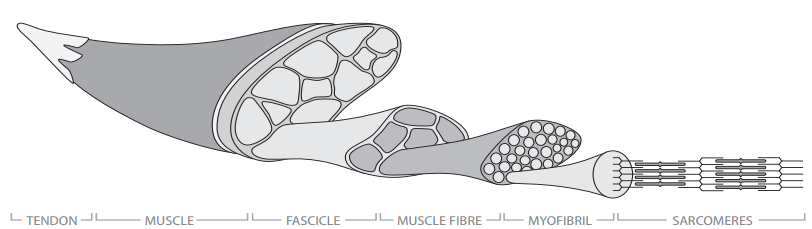
\includegraphics[width=0.7\linewidth]{muscle_struct}
	\caption[Строение мышцы]{Строение мышцы}
	\label{fig:musclestruct}
\end{figure}

\par Мышечное брюшко окружено плотным и прочным покровом, который называется фасцией. Внутри же содержаться различной толщины пучки мышечных волокон, каждое из которых образованно параллельными миофибриллами. Миофибрилы являются нитевидными образованиями, состоящими из саркомеров. 
\par Все соединительные образования мышцы с мышечного брюшка переходят на сухожильные концы. Они состоят из плотной волокнистой соединительной ткани, коллагеновые волокна которой лежат между мышечными волокнами, плотно соединяясь с их сарколеммой (оболочкой мышечных волокон).
\par Значительное влияние на работу мышц оказывает направление их волокон. По этому признаку выделяют: мышцы с параллельными, поперечными и косыми волокнами. Косые в свою очередь делятся на одноперистые, если присоединяются к сухожилию с одной стороны, и двуперистые, если с двух сторон. Данные особенности в строении определяют то, насколько подвижными являются мышцы и какую силу они могут производить.
\par При сокращении центральная нервная система подаёт сигнал в мышцы, в результате которого нити саркомеров скользят друг вокруг друга, что приводит к укорачиванию саркомера~\cite{muscle_03}. Скольжение нитей вызывает мышечное напряжение, что является основным вкладом саркомера, так как именно это действие даёт мышцам их физическую силу. 
\par Задачей программы является представление визуальной модели мышц, которая позволила бы наблюдать за процессом их сокращения, благодаря чему было бы проще изучить их строение и основные принципы работы.

\section{Способы моделирования мышечных сокращений}
\label{sec:muscle_meth}
Существуют различные способы представления мышечных сокращений. В зависимости от принципов, лежащих в основе каждого из методов, их можно разделить на: геометрически-основанные и физически-основанные~\cite{diff_methods}. В геометрически-основанных подходах большее внимание уделяется анимации расширения и укорачивания, в то время как физический аспект сокращения не учитывается. Они успешно моделируют простые мышцы, но им недостаёт реализма в физиологическом или биомеханическом аспектах. В противовес к таким подходам ставятся физически-обоснованные подходы, в которых рассматриваются сложные проблемы, включающие в себя динамику мышц и свойства тканей. Чтобы смоделировать физически-корректную модель мышц решают две проблемы: определение силы сокращения и представление изменения мышечной геометрии.

\subsection{Использование деформируемых эллипсоидов для аппроксимации мышц}
\label{subsec:elypsoids}
Идея данного метода заключается в использовании параметрических эллипсоидов в качестве базовых примитивов для моделирования мышц. Три главные оси отрегулированы так, чтобы представлять выпуклость мышечного брюшка, в то время как объём сохраняется за счёт использования определённых соотношений между этими тремя осями~\cite{scheepers97}. Чтобы симулировать изометрические сокращения мышц, вводится параметр напряжённости t, в связи с чем соотношение шириной и высотой эллипсоида рассчитывается по формуле:
\begin{equation}\label{r_eq}
r = (1 - t)r_{n} + ktr_{n} = (1 - t + kt)r_{n}
\end{equation}
где k - параметр контроля напряжённости, который регулирует, насколько выпукла мышца, $r_{n} = \frac{a_{n}}{b_{n}}$ - соотношение ширины к высоте в расслабленном состоянии. 
\par Для представления более сложных форм могут использоваться сразу несколько эллипсоидов, расположенных на определённой кривой, или же прямой путь между концами мышцы может быть заменён кривой Безье, представляющей направление силы, и эллипсоидами разных размеров, расположенных вдоль этой кривой~\cite{scheepers97}

\subsection{Обобщённая цилиндрическая модель}
\label{subsec:cylinder}
Аналогичным подходом является представление мышц, основанное на деформируемых цилиндрах. Ось цилиндра - кривая, вдоль которой расположены эллиптические срезы. Именно на их основе строится полигональный меш~\cite{Wilhelms97}. Подразумевается, что каждый радиус, позиция и наклон каждого эллипса могут быть изменены, что позволяет формировать мышцы сложной формы.
\par При сокращении ширина и толщина внутренних срезов увеличивается в соотношении $\sqrt{l_{n} / l}$, где $l_{n}$ - длина в расслабленном состоянии, а $l$ - текущая длина. За счёт этого поперечная область расширяется, если мышцы становятся короче, и сужается, если удлиняются.
\par Другим способом является задание мышцы, используя модифицированный обобщенный цилиндр, определяемый с помощью кривой толщины $C_{T}(t)$ вдоль кривой наклона $C_{S}(t)$~\cite{ramos}. $C_{S}(t)$ это трёхмерный сплайн, представляющий профиль мышцы. Он определяется двумя точками - источником O и целью I. $C_{T}(t)$ - одномерная функция, представляющая толщину мышцы от t. Срез мышцы в t определяется эллипсом, расположенным вдоль $C_{S}(t)$, толщина которого получена из $C_{T}(t)$. Чтобы избежать пересечения секций и упростить сохранение объёма, поперечное сечение всегда расположено перпендикулярно линии действия, лежащей на главной оси мышечной формы.

\subsection{Mass-spring System}
\label{subsec:MSS}
Объект моделируется набором точечных масс, связанных между собой невесомыми пружинами. Такая модель может быть расширена при добавлении различных типов сил, применяемых к пружине, таких как угловую или силу сжатия. Линии, называемые линиями действия, используются для вычисления силы, прилагаемой к костям при сокращении~\cite{nedel}. В зависимости от формы и сложности их строения, мышцы могут быть представлены одной или несколькими линиями действия, кроме того каждая линия может быть полилинией.
\par Такой подход позволяет разделить модель на 2 уровня: линию действия, задаваемую точками начала и конца, и форму мышцы. Важной частью формирования данной модели является установление соответствия между точками массы и формой мышц. Для этого каждая точка должна быть расположена между двумя соседними в горизонтальном и двумя другими в вертикальном смысле. Чтобы модель мышц удовлетворяла этим требованием, необходимо несколько изменять форму ее меша. Из-за чего происходят потери в качестве. Кроме того, такой подход применим только к мышцам, обладающим вытянутой формой~\cite{nedel}.
\par Преимуществом модели, использующей точки масс является возможность рассчитать силу сокращения для каждой точки, используя формулу, в которой сила упругости, действующая на неё определяется суммой сил, с которыми пружины, связывающие ее с 4 соседями, притягиваются:
\begin{equation}\label{mss_01}
f_{result}(x_{i})=f_{elasticity}(x_{i})+f_{curvuture}(x_{i})+f_{constraints}(x_{i})
\end{equation}
\begin{equation}\label{mss_02}
f_{elasticity}=\sum_{j=0}^{3}f_{spring_{j}}(x_{i})=\sum_{j=0}^{3}-ks(x_{i}-x_{rest})
\end{equation}
где $ks$ - коэффициент упругости пружины, $x_{i}$ - экстремум её колебания, $x_{rest}$ - расслабленное положение этого экстремума. Для формирования искривлённости мышцы вводятся дополнительные пружины, соединяющие не соседние точки.

\subsection{Метод конечных элементов}
\label{subsec:FEM}
В основе этого метода лежит разбиение тела на набор конечных элементов, например гексаэдров или тетраэдров. Перемещения и положения в элементе аппроксимированы с помощью интерполяционных функций:
\begin{equation}\label{eq:FEM}
\Phi(x)\approx\sum_{i}h_{i}(x)\Phi_{i}
\end{equation}
где $h_{i}$ - интерполяционная функция для элемента, содержащего x и $\Phi_{i}$ - скалярный вес, сопоставленный с $h_{i}$ Такой подход часто применяется для представления твёрдых упругих тел. \par Одним из способов применения метода конечных элементов является модель, в которой кроме полигонального представления мышц, применяются двадцати-вершинные блоки, являющиеся "двигателем" модели~\cite{chen}. После чего для сетки каждого блока формируются динамические уравнения равновесия. Механическая модель мышц используется для приложения сил к вершинам блоков,  после чего их форма динамически меняется, что в свою очередь оказывает влияние на полигоны. Для двадцати-вершинного блока уравнение равновесия имеет вид:
\begin{equation}\label{key}
M\ddot{u}+C\dot{u}+Ku=R(t)
\end{equation}
Для тела, имеющего n узловых точек, u - это вектор размерности 3n, отображающий расположение вершин, M, C и K матрицы размерности 3n*3n, описывающие массу, затухание и жёсткость между точками внутри тела, и R - это вектор сил, прилагаемых к каждой вершине, размерностью 3n.
\par Чтобы симулировать мышечное сокращение, в вершинах добавляются генераторы силы, которые действуют вдоль продольного направления мышц. В двадцати-вершинном блоке расположено 8 таких генераторов.

\subsection{Метод конечных объёмов}
\label{subsec:FVM}
Аналогично предыдущему методу метод конечных объёмов разбивает модель на множество элементов. Однако для расчёта прилагаемых сил объёмные интегралы трансформируют в интегралы по площади, используя формулу Гаусса-Остроградского. Эти условия затем расцениваются как потоки на поверхности каждого конечного объёма. Эта модель используется для представления деформации скелетных мышц, и считается, что она более производительна и обладает меньшим потреблением памяти, чем метод конечных элементов~\cite{teran}.
\paragraph{Вывод} было решено использовать обобщённую цилиндрическую модель для аппроксимации мышц, так как она позволит 

\section{Выбор методов моделирования}
\label{sec:model_meth}
Выделяют три основных типа моделей: каркасные, граничные и сплошные~\cite{nikulin}. Каркасная конструкция в виде проволочной сетки является простейшим способом передачи формы объёмного тела. Проволочные модели дают возможность быстро визуализировать низко детализированные объекты.
\par Граничная модель представляет объект системой элементов, создающих его границы. Для задания границ могут использоваться аналитическая и векторная полигональная модели~\cite{porev}. Первая - это такая модель, в которой для описания поверхности используются математические формулы. Например в виде функций двух аргументов $ z = f(x, y)$ или уравнением $F(x, y, z) = 0$.
\par Преимущества параметрического описания - легко описывать поверхности, которые отвечают неоднозначным функциям, лёгкость процедуры расчёта координат каждой точки поверхности, нормали; небольшой объём информации для описания достаточно сложных форм.
\par К недостаткам относятся следующие: невозможность в большинстве случаев применения данной формы непосредственно для построения изображения; некоторые сложные формулы описания могут медленно вычисляться на компьютере~\cite{porev}.
\par Другим способом задания пространственных объектов является векторная полигональная модель. Ее основными элементами являются: вершины, отрезки прямых, полилинии, полигоны, полигональные поверхности. Векторная полигональная модель считается наиболее распространённой в современных системах трёхмерной графики. Положительными чертами векторной полигональной модели являются:
\begin{itemize}
	\item удобство масштабирования объектов, диапазон которого определяется точностью аппроксимации;
	\item небольшой объём данных для описания простых поверхностей, аппроксимируемых плоскими гранями;
	\item необходимость вычислять только координаты вершин при преобразованиях систем координат или перемещении объектов.
\end{itemize}
Недостатки:
\begin{itemize}
	\item аппроксимация плоскими гранями приводит к погрешности моделирования;
	\item сложные алгоритмы выполнения топологических операций, таких, например, как разрезы.
\end{itemize}
\par Сплошная модель включает в объект как граничные, так и внутренние точки. Это позволяет представлять сложный объект в виде композиции простых составляющих - кубов, сфер, конус и т.д. Простейшая декомпозиция заключается в разбиении пространства на кубические или сферические ячейки, называемые вокселами, и установления состояния каждой ячейки - свободна она или занята объёмом тела. Преимущества такой модели:
\begin{itemize}
	\item позволяет достаточно просто описывать сложные объекты и сцены;
	\item простое выполнение топологических операций над отдельными объектами и сценой в целом.
\end{itemize}
Недостатки:
\begin{itemize}
	\item большое количество информации, необходимой для представления объемных данных;
	\item значительные затраты памяти ограничивают разрешающую способность, точность моделирования;
	\item при увеличении или уменьшении изображения возникают проблемы, например при увеличении ухудшается разрешающая способность.
\end{itemize}
\paragraph{Вывод:} выбирая между методами моделирования, было решено использовать полигональный, так как он является более экономичным по памяти, чем воксели. Кроме того, они такое представление позволяет легко изменять форму модели, что положительно влияет на производительность, при анимации сокращения мышц. 

\section{Выбор метода морфинга}
\label{sec:morph}
Морфинг - это интерполяционная техника, используемая для создания плавной трансформации одного изображения в другое~\cite{volume_morph}. Для изображений, сгенерированных на основе трёхмерных моделей, существует альтернатива морфингу самого изображения: трёхмерный морфинг, который формирует промежуточные модели на основе заданных, они затем используются, чтобы произвести последовательность изображений. Преимуществами такого подхода являются:
\begin{itemize}
	\item промежуточные формы не зависят от точки обзора и свойств освещения;
	\item двумерным техникам не достаёт информации о пространственной конфигурации модели, в связи с чем они не могут корректно обрабатывать изменения в освещении и видимости~\cite{volume_morph}.
\end{itemize}
Трёхмерные техники могут применяться моделям, заданным объёмами или гранично описанным - мешами. Меш $M$ можно описать парой $(K, V)$, где $K$ - это набор, отображающий связь вершин, рёбер и граней и $V = (v_{1},\dots,v_{n})$ - описывает геометрическое положение вершин в $R^{d}$~\cite{alexa}. Обычно, морфинг применяются к двум заданным мешам $M_{0}=(K_{0},V_{0})$ и $M_{1}=(K_{1},V_{1})$. Целью является построение группы мешей $M(t)=(K,V(t)),t\in[0,1]$, генерация ее обычно выполняется за три последовательных шага~\cite{alexa}:
\begin{enumerate}
	\item Поиск соответствия между мешами. А именно сопоставление вершин, лежащих в исходной фигуре, с вершинами целевой фигуры.
	\item Формирование новой, последовательной связности $K$ для каждого вершины на основе геометрических позиций $V(0), V(1)$. Традиционный подход к этой проблеме заключается в создании надмножества $K_{0}$ и $K_{1}$. Однако, в некоторых случаях ремешинг может быть полезен в случае, когда исходные меши обладают разными разрешениями.
	\item Создание путей $V(t),t\in]0,1[$ для вершин. Данный шан обладает некоторыми ограничениям: в большинстве случаев не ожидается, что форма будет разрушаться или самопересекаться, и, как правило, ожидается, что пути будут гладкими. Самый простой способ, получить такие пути - это линейная интерполяция координат вершин. При заданном параметре $t$ координаты интерполированной формы вычисляются как:
	\begin{equation}
	V(t)=(1-t)V(0)+tV(1)
	\end{equation}
	Такая интерполяция даст хорошие результаты, если формы одинаково ориентированны и в некоторой степени похожи.
\end{enumerate}
\par Для определения, в какое положение должен перейти тот или иной полигон, можно использовать, например, методы ближайшего соседа и сортировки рёбер~\cite{morphing}. Идея метода ближайшего соседа заключается в поиске наименьшего расстояния между треугольниками, но вместо трёхмерного пути, который прошли бы центры этих рёбер при перемещении, рассматриваются возможные перестановки вершин и из них выбирается наименьшее. Так, для двух треугольников возможно 6 перестановок, но 3 из инвертирует нормаль к полигону, в связи с чем рассматриваются 3 оставшиеся, из них выбирается та, которая минимизирует путь, необходимый для перемещения из одного набора вершин в другой. Однако такой метод не гарантирует, что все сопоставления будут уникальными.
\par Другой метод - сортировка рёбер, в нем каждый треугольник рассматривается как узел а каждое сопоставление между двумя треугольниками - ребро. И поскольку определение соответствия выполняется между двумя множествами источников и целей, проблема сводится к формированию двудольного графа, который соединяет все вершины, и каждую только один раз. В таком случае алгоритм состоит из следующих шагов:
\begin{itemize}
	\item Сформировать полный взвешенный биграф, в котором вес - расстояние между двумя полигонами, как в методе ближайшего соседа.
	\item Упорядочить все ребра по весу.
	\item Для каждого ребра, в сортированном списке, если обе вершины свободны, то установить соответствие, иначе выбрать следующее.
\end{itemize}
В результате для каждого полигона будет однозначно установлен полигон, в который он должен перейти.

В случае, когда морфинг применяется к объёмно-заданной модели, проблема может быть сформирована так - даны два объёма S и T, необходимо произвести последовательность промежуточных объёмов, удовлетворяющим условиям реалистичности и плавности~\cite{volume_morph}. Создание этих состояний разбивается на два этапа:
\begin{itemize}
	\item Искривление - S и T искривляются, чтобы получить объёмы S' и T'. Для этого могут задаваться пары элементов, один элемент из исходного и один в результирующим объёмах. Необходимо задать несколько таких пар, которые определят общее соответствие между двумя объектами. Эти пары объектов взаимодействуют как магниты, формирующие податливые объёмы~\cite{volume_morph}.
	\item Смешивание может выполняться перекрёстным растворением объёмов или же их двумерных изображений. Под смешиванием объемов подразумевается интерполяция вокселей, из которых они состоят.
\end{itemize}
\paragraph{Вывод:} было решено использовать трёхмерный морфинг на основе мешей с использованием метода сортировки рёбер для установления соответствий, что также связано с ранее выбранным методом полигонального представления модели, так как это позволит получить плавную анимацию с учётом освещения и видимости. Кроме того, этот метод даст хорошие результаты, поскольку форма мышц при сокращении не слишком сильно изменяется.

\section{Анализ методов удаления невидимых граней}
\label{sec:inv_edge}

\paragraph{Алгоритм Роберста} работает в объектном пространстве с выпуклыми телами. Если имеются невыпуклые тела, то их сначала необходимо разбить на выпуклые~\cite{rogers}. В алгоритме в первую очередь удаляются те ребра и грани, которые экранируются самим телом, затем каждое из видимых рёбер каждого тела сравнивается с каждым из оставшихся тел для определения того, какая его часть или части экранируются другими телами.
\par Недостатком алгоритма Робертса является то, что теоретически его вычислительная ёмкость растёт как квадрат числа объектов. Однако существуют модификации алгоритма с использованием приоритетной сортировки вдоль оси z и простых габаритных или минимаксных тестов~\cite{rogers}, которые позволяют свести вычислительную сложность к почти линейной зависимости от числа объектов.

\paragraph{Алгоритм Варнока} работает в пространстве изображений. Идея алгоритма заключается в том, что рассматривается окно и решается вопрос о том, пусто оно или нет его содержимое достаточно просто для визуализации~\cite{rogers}. В противном случае окно разбивается на более маленькие области, для которых снова решается этот вопрос. Предполагается, что если размер окна в результате его разбиения стал совпадать с одним пикселем, но при этом оно содержит не один многоугольник, то необходимо визуализировать тот из них, у которого максимальное значение координаты Z.
\par Недостатком алгоритма может являться необходимость проведения большого количества разбиений, что негативно скажется на временной эффективности.

\paragraph{Алгоритм, использующий Z-буфер} является одним из простейших алгоритмов удаления невидимых поверхностей~\cite{rogers}. Он работает в пространстве изображения. 
\par Суть алгоритма заключается в использовании Z-буфера, в котором запоминается координата z каждого видимого пикселя, в то время как буфер кадра используется для запоминания атрибутов каждого пикселя. В процессе работы глубина очередного пикселя сравнивается с глубиной, находящейся в Z-буфере, и в результате сравнения либо заносится в этот буфер, или никаких действий не производится.
\par Преимуществом данного алгоритма является его простота. Кроме того, он позволяет работать со сценами любой сложности, делая тривиальной визуализацию пересечений сложных поверхностей. Алгоритм обладает не более чем линейной вычислительной трудоёмкостью.
\par Недостатком же алгоритма является необходимость хранить Z-буфер, что увеличивает затраты по памяти, однако для современных компьютеров они являются незначительными~\cite{rogers}.

\paragraph{Алгоритм трассировки лучей} - метод грубой силы~\cite{rogers}. Главной идеей данного метода является запуск луча для каждого пикселя картинной плоскости, для каждого луча происходит проверка на пересечение с каждым из объектов сцены, после чего пересечения упорядочиваются по глубине. Пересечение с максимальным значением z представляет видимую поверхность для данного пикселя.
\par К достоинствам алгоритма можно отнести то, что вычислительная сложность метода линейно зависит от сложности сцены. В результате выполнения алгоритма получается очень реалистичное изображение. А также метод даёт возможность создания гладких объектов без аппроксимации их примитивами.
\par Однако для получения такого изображения необходимо создать огромное количество лучей, проходящих через сцену, и необходимость нахождения пересечения с каждым из объектов, что негативно сказывается на скорости работы программы.
\par Чтобы уменьшить количество искомых пересечений производится поиск пересечения луча с объёмной оболочкой рассматриваемого объекта. Если оно не найдено, то нет необходимости в поиске пересечения с объектом. В качестве оболочки можно применять параллелепипед или сферу.
\paragraph{Вывод:} было решено использовать алгоритм, использующий Z-буфер, поскольку его реализация проще, чем у других алгоритмов, в то время как его вычислительная трудоёмкость сохраняется линейной. И, как уже было отмечено раньше, затраты памяти, связанные с хранением Z-буфера, больше, чем у других алгоритмов, они всё же незначительны для современных вычислительных машин.


\section{Анализ моделей освещения}
\label{sec:light}
Простая модель освещения ограничивается отображением света, исходящего от явных точечных источников. В ней не учитываются взаимодействия объектов сцены между собой, но учитывается диффузное отражение света. Интенсивность света, отражённого предметом вычисляется по формуле:
\begin{equation}\label{lambert}
I = I_{a}k_{a} + I_{l}k_{d}\cos \theta \qquad 0\leq\theta\leq\pi/2
\end{equation}
Глобальная модель описывает освещение, учитывая взаимное влияние объектов сцены. Она рассматривает многократное отражение и преломление света, рассеянное освещение. Для этого отслеживается путь луча до тех пор, пока он не покинет сцену или его энергия не станет достаточно малой, чтобы не учитывать ее. Глобальная модель освещения позволяет получить более реалистичное изображение.
\paragraph{Вывод:} для визуализации мышц можно пренебречь преломлением и бликами, так что было решено использовать простую модель освещения, используя формулу Ламберта. Кроме того использование такой модели позволит выиграть в производительности.

\section{Анализ методов закраски}
\label{sec:color}
\paragraph{Метод простой закраски-} его идея заключается в том, что для каждой грани объекта находится вектор нормали, с помощью которого в соответствии с выбранной моделью освещения вычисляется значение интенсивности, с которой закрашивается вся грань.
\par Метод простой закраски обладает наилучшим быстродействием, однако все пиксели грани обладают одинаковой интенсивностью, в связи с чем сцена может выглядеть нереалистично.

\paragraph{Метод Гуро} позволяет получить более сглаженное изображение, чем простая закраска. Такой результат получается за счёт билинейной интерполяции интенсивностей в пределах одной сканирующей строки.
\par Недостатками метода Гуро является появления полос Маха в связи с тем, что такой метод интерполяции не обеспечивает непрерывности изменения интенсивности, а также то, что некоторые рёбра могут казаться сглаженными.

\paragraph{Метод Фонга} требует больших вычислительных затрат, чем закраска по Гуро. Идея такой закраски заключается в интерполировании вектора нормали вдоль сканирующей строки, который затем используется в модели освещения для расчёта интенсивности.

\paragraph{Вывод:} выбирая между методами закраски было решено использовать метод Гуро, который позволяет получить результат лучше, чем метод простой закраски, и быстрее, чем метод Фонга. Кроме того, в результате закраски методом Гуро ребра будут выглядеть плавными, что является преимуществом для модели мышц.

\label{sec:color}

\chapter{Конструкторский раздел}
\label{cha:design}
В этом разделе будут рассмотрены требования к программе и схемы для реализации алгоритмов, математические расчёты.
Программа должна предоставлять возможность:
\begin{itemize}
	\item загружать модель мышц;
	\item вращать и перемещать загруженную модель;
	\item визуализировать мышечные сокращения;
	\item задавать степень сокращения;
	\item добавлять и перемещать источники освещения.
\end{itemize}

\section{Общий алгоритм работы программы}
\label{sec:general}
Алгоритм работы программы можно описать следующими шагами.
\begin{enumerate}[1.]
	\item Загрузить модель из файла.
	\item Сформировать модель сокращённой мышцы, учитывая степень сокращения.
	\item Сформировать промежуточные меши:
	\begin{enumerate}
		\item для каждого промежуточно меша закрасить объект используя простую модель освещения;
		\item заполнить буфер глубины и экранный буфер, применяя алгоритм z-буфер;
		\item вывести заполненный экранный буфер.
	\end{enumerate}
\end{enumerate}
На рисунках \ref{fig:01a-0} и \ref{fig:02a0} приведены IDEF0 диаграммы, которые представляют организацию работы программы.
\begin{sidewaysfigure}
	\begin{figure}[H]
		\centering
		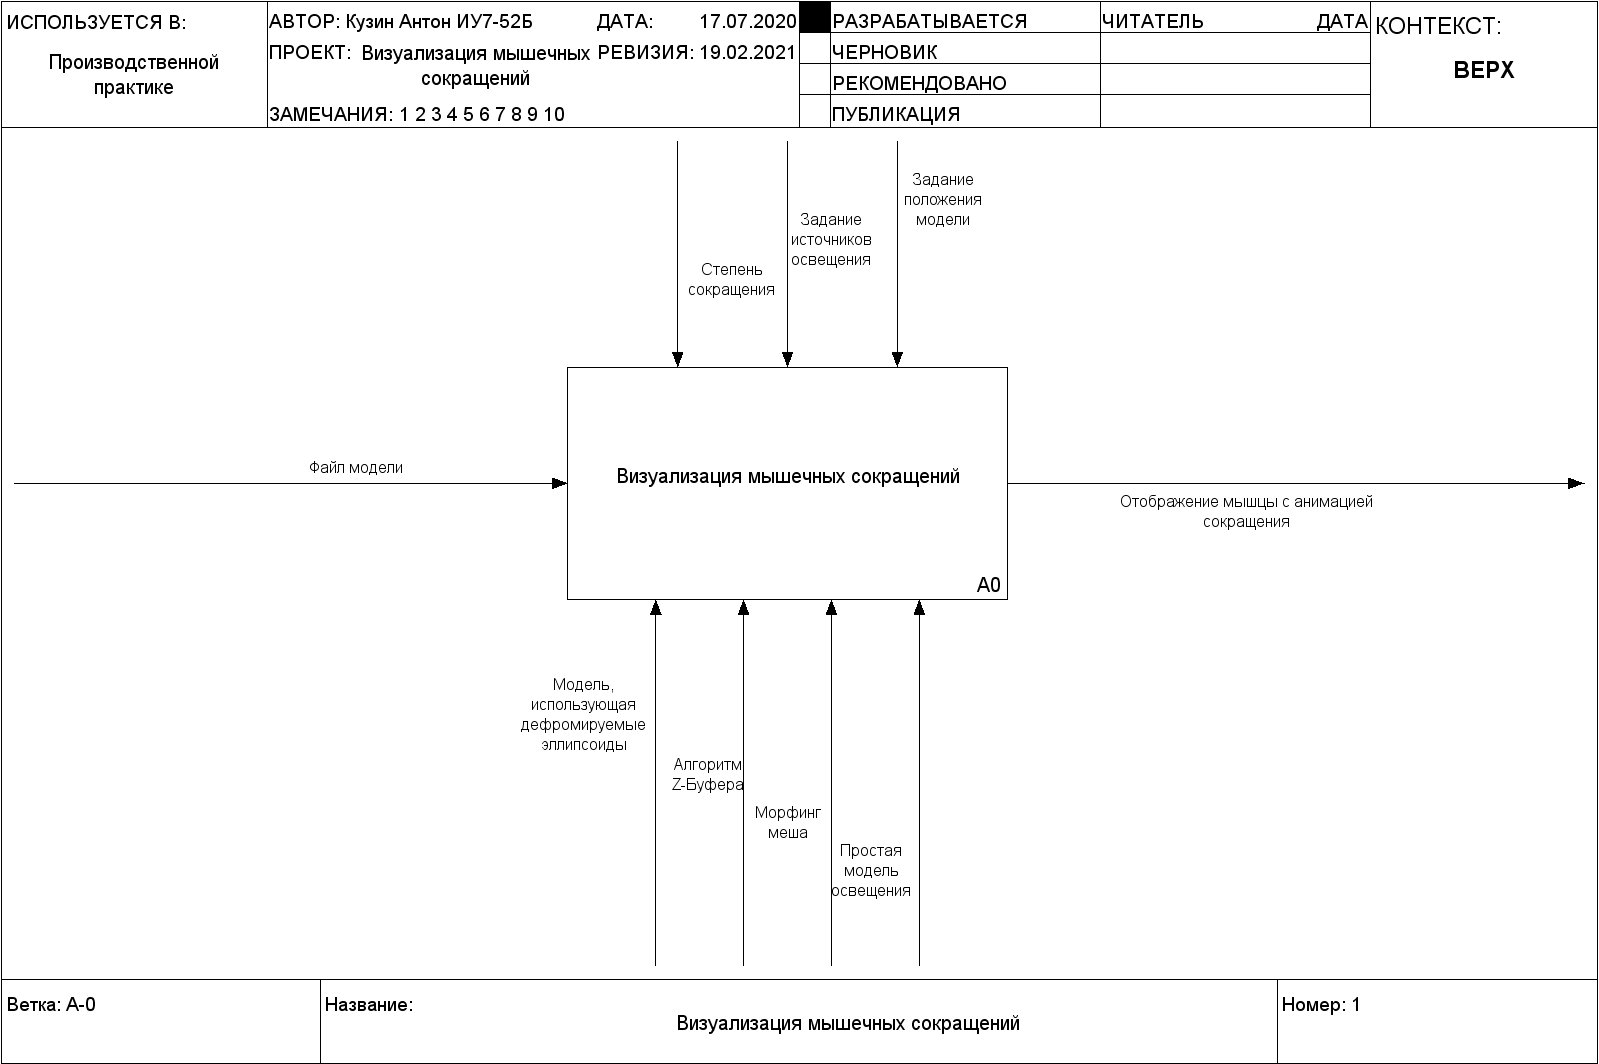
\includegraphics[height=0.5\paperheight]{images/01_A-0}
		\caption[IDEF0 диаграмма, блок А0]{IDEF0 диаграмма работы программы}
		\label{fig:01a-0}
	\end{figure}
\end{sidewaysfigure}
\begin{sidewaysfigure}
	\begin{figure}[H]
		\centering
		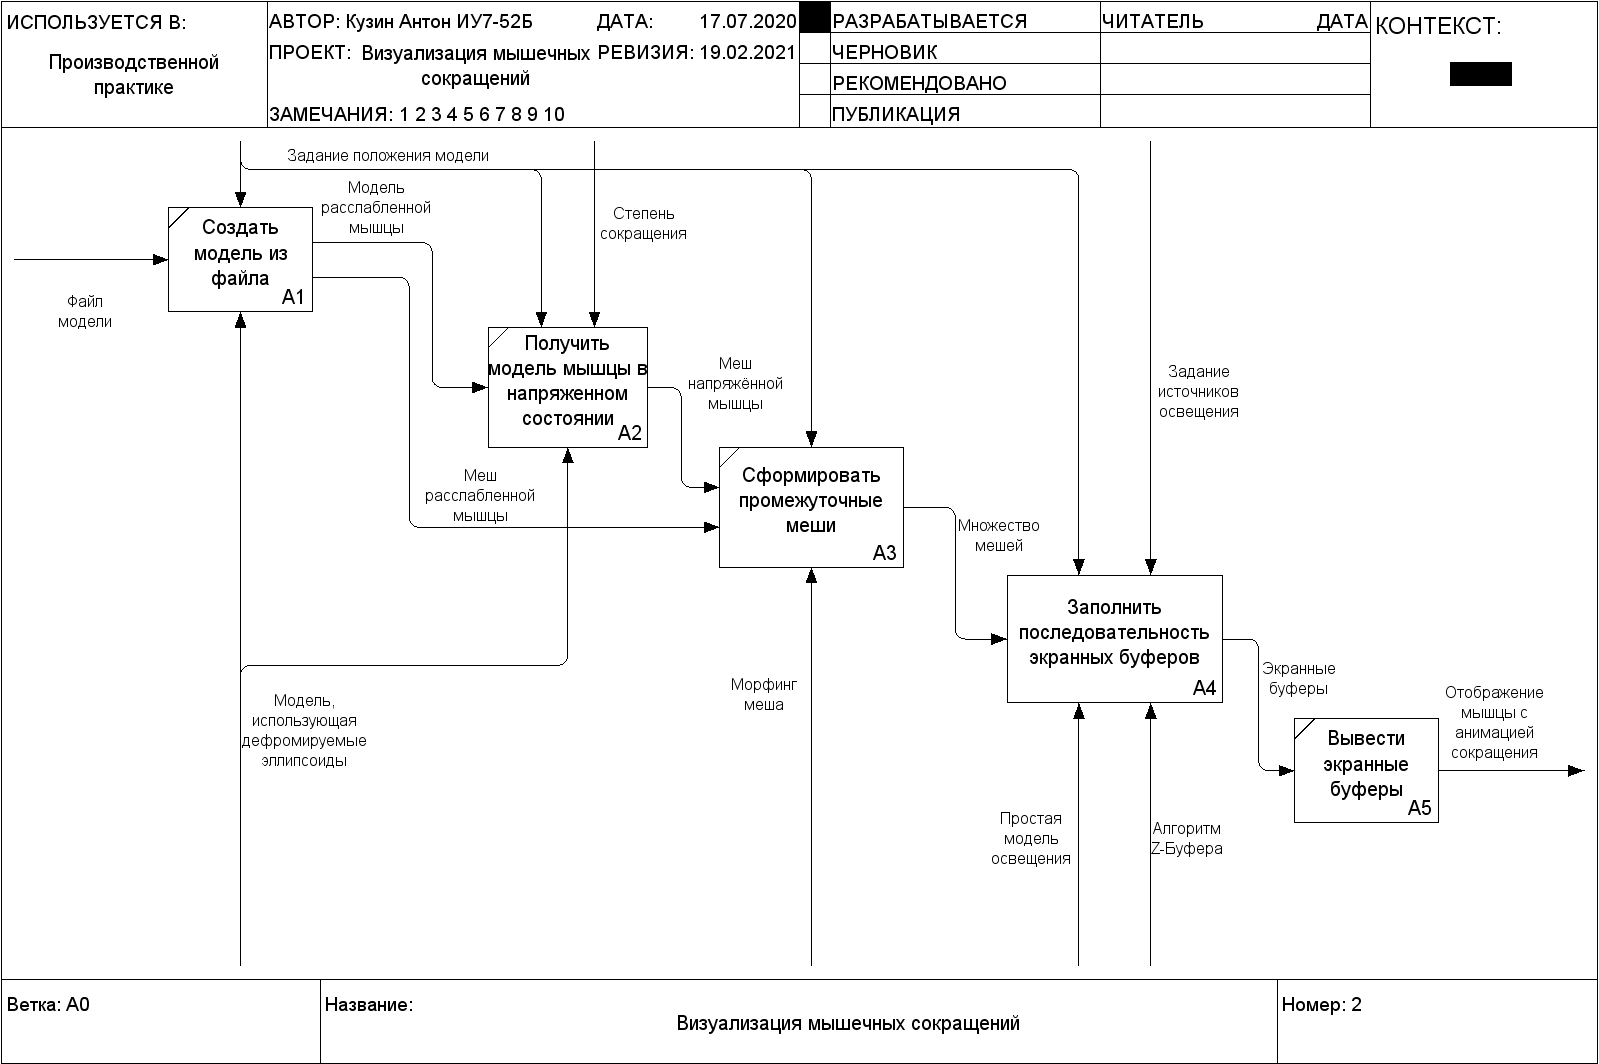
\includegraphics[height=0.5\paperheight]{images/02_A0}
		\caption[Последовательность действий для отображения анимации сокращения мышцы]{Последовательность действий для отображения анимации сокращения мышцы}
		\label{fig:02a0}
	\end{figure}
\end{sidewaysfigure}

\section{Реализуемые алгоритмы алгоритмы}
\label{sec:algs}
\paragraph{Модель скелетных мышц}
В качестве модели аппроксимации скелетных мышц было решено использовать деформируемые эллипсоиды. Для представления сокращения параметры эллипсоида задаются с помощью математических уравнений~\cite{scheepers97}, что позволяет сохранять объем и соотношение между высотой и шириной мышцы. Объем рассчитывается по формуле:
\begin{equation}
	v = \frac{4\pi abc}{3}
\end{equation}
Полагая $l'$ новой длиной мышцы, $r=\frac{a}{b}$, новые параметры вычисляются по формулам:
\begin{equation}
	c'=\frac{l'}{2}
\end{equation}
\begin{equation}
	b'=\sqrt{\frac{3v}{4\pi rc'}}
\end{equation}
\begin{equation}
	a'=b'r
\end{equation}
Для визуализации изометрического сокращения мышцы соотношение r пересчитывается по формуле:
\begin{equation}
	r=(1-t+kt)r_n
\end{equation}
где $r_n$--соотношение $\frac{a}{b}$ в расслабленном состоянии, $t$--степень напряжённости $t\in [0,1]$, $k$--параметр контроля напряжения, который регулирует степень сжатия.

\par Для изображения моделей мышц, аппроксимируемых эллипсоидами, алгоритмом, использующим Z-буфер, необходимо представить её с помощью полигонов. Алгоритм, триангулирующий эллипсоид, который задан параметрами $a, b$ и $c$, можно описать следующими шагами:
\begin{enumerate}[1.]
	\item Построить куб в начале координат.
	\item Представить его в виде треугольных полигонов.
	\item Выполнять рекурсивное разбиение полигонов, путём создания вершин в середине каждого из 3-х рёбер.
	\item Нормализовать каждую вершину.
	\item К полученной сфере применить преобразования, умножив координаты точек на параметры a, b и c эллипсоида.
\end{enumerate}
\par Увеличение глубины рекурсии создаст большее число полигонов, что позволит сделать изображение более реалистичным, однако увеличит время необходимое на его обработку.

\paragraph{Алгоритм z-буфера}
в общем виде может быть описан последовательностью таких шагов:
\begin{enumerate}[1.]
	\item Заполнить буфер кадра фоновым значением интенсивности или цвета.
	\item Заполнить z-буфер минимальным значением z.
	\item Преобразовать каждый многоугольник в растровую форму в произвольном порядке:
	\begin{enumerate}
		\item Для каждого пикселя в многоугольнике вычислить его глубину z.
		\item Сравнить глубину z со значением z в буфере в этой же позиции. Если z > Zбуфер, то записать атрибут этого пикселя в буфер кадра и заменить Zбуфер на z.
	\end{enumerate}
\end{enumerate}

\paragraph{Простая модель освещения} интенсивность рассчитывается по закону Ламберта c учётом рассеянного освещения, представленного константой:
\begin{equation}\label{lambert2}
I = I_{a}k_{a} + I_{l}k_{d}\cos \theta \qquad 0\leq\theta\leq\pi/2
\end{equation}
$I$ - интенсивность отражённого света, $I_{i}$ - интенсивность точечного источника, $k_{d}$ - коэффициент диффузного отражения ($0\leq k_{d}\leq 1$), $\theta$ - угол между направлением света и нормалью к поверхности, $I_{a}$ - интенсивность рассеянного света, $k_{a}$ - коэффициент диффузного отражения рассеянного света($0\leq k_{a}\leq 1$).

\paragraph{Морфинг меша} можно разделить на два этапа: установление соответствия между полигонами начального и конечного состояний модели и интерполяция положения вершин. На рисунке \ref{fig:morphingalg} представлен алгоритм морфинга мешей, следует отметить что для установления связи между полигонами начала и конца не производится никаких вычислений, а каждому i-ому полигону начала в соответствие ставится i-ый полигон конца, это связано с тем, что объект источника и объект цели имеют одинаковую форму и одинаковое количество полигонов, в связи с чем предполагается, что для того, чтобы не нарушить целостность объекта необходимо сопоставить их в том же порядке.
\begin{figure}[H]
	\centering
	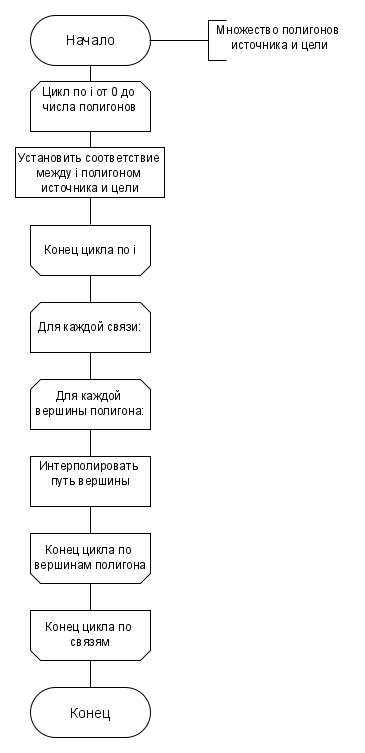
\includegraphics[width=0.7\linewidth]{images/morphing_alg}
	\caption[Алгоритм морфинга]{Алгоритм морфинга}
	\label{fig:morphingalg}
\end{figure}

\section{Вывод}
\label{sec:conc_constr}
В этом разделе были рассмотрены требования к программе, общий алгоритм ее работы, представлены схемы для реализации выбранных алгоритмов и математические формулы.

%\chapter{Технологический раздел}
\label{cha:impl}
В данном разделе будут представлены средства реализации, разработанные алгоритмы и интерфейс.

\section{Средства реализации}
\label{sec:realisation}
В качестве языка программирования был выбран Python так как это мощный объектно-ориентированный язык, с которым я был знаком, что сократит время написания программы и упростит разработку.
\par В качестве среды разработки была выбрана "PyCharm Community Edition", а для представления пользовательского интерфейса библиотека PyQt5.

\section{Описание структуры программы}
\label{sec:structure}
\paragraph{Описание основных модулей программы}
\begin{itemize}
	\item main.py -- загружает интерфейс и запускает программу;
	\item window.py -- содержит класс интерфейса;
	\item sceneinterface.py -- содержит класс SceneInterface, выступающий в качестве посредника между сценой и интерфейсом;
	\item scene.py -- содержит класс сцены, основной класс, в котором находятся объекты и источники света;
	\item commands.py -- содержит классы команд, которые влияют на сцену;
	\item controlmanager.py -- содержит классы менеджеров, отвечающие за выполнение сложных команд, таких как отрисовка и загрузка моделей;
	\item builder.py -- содержит класс Builder, отвечающий за чтение файла и создание объекта модели;
	\item builddirector.py -- содержит класс, контролирующий создание объекта;
	\item drawer.py -- содержит классы QDrawer и BaseDrawer, которые предоставляют методы отрисовки на самом низком уровне;
	\item drawerfactory.py -- содержит классы DrawerFactory и QDrawerFactory, целью которых является создание объекта Drawer;
	\item baseobject.py -- содержит класс базового объекта, точки и вектора;
	\item invisibleobject.py -- содержит класс камеры и источника света;
	\item visibleobject.py -- содержит класс полигона;
	\item visitor.py -- содержит методы, применяемые к разным объектам сцены, а именно перемещение и поворот;
	\item visualizer.py -- содержит методы, отвечающие за взаимодействие с drawer-ом;
	\item musclemodel.py -- содержит класс эллипсоида, прямой мышцы и сложной мышцы;
\end{itemize}
На рисунке \ref{fig:scheme} представлена диаграмма классов, из неё видно разделение на отдельные модули, что позволяет изменять и дополнять некоторые из них независимо от других, благодаря чему программу будет проще обновлять при необходимости.
\begin{figure}[H]
	\centering
	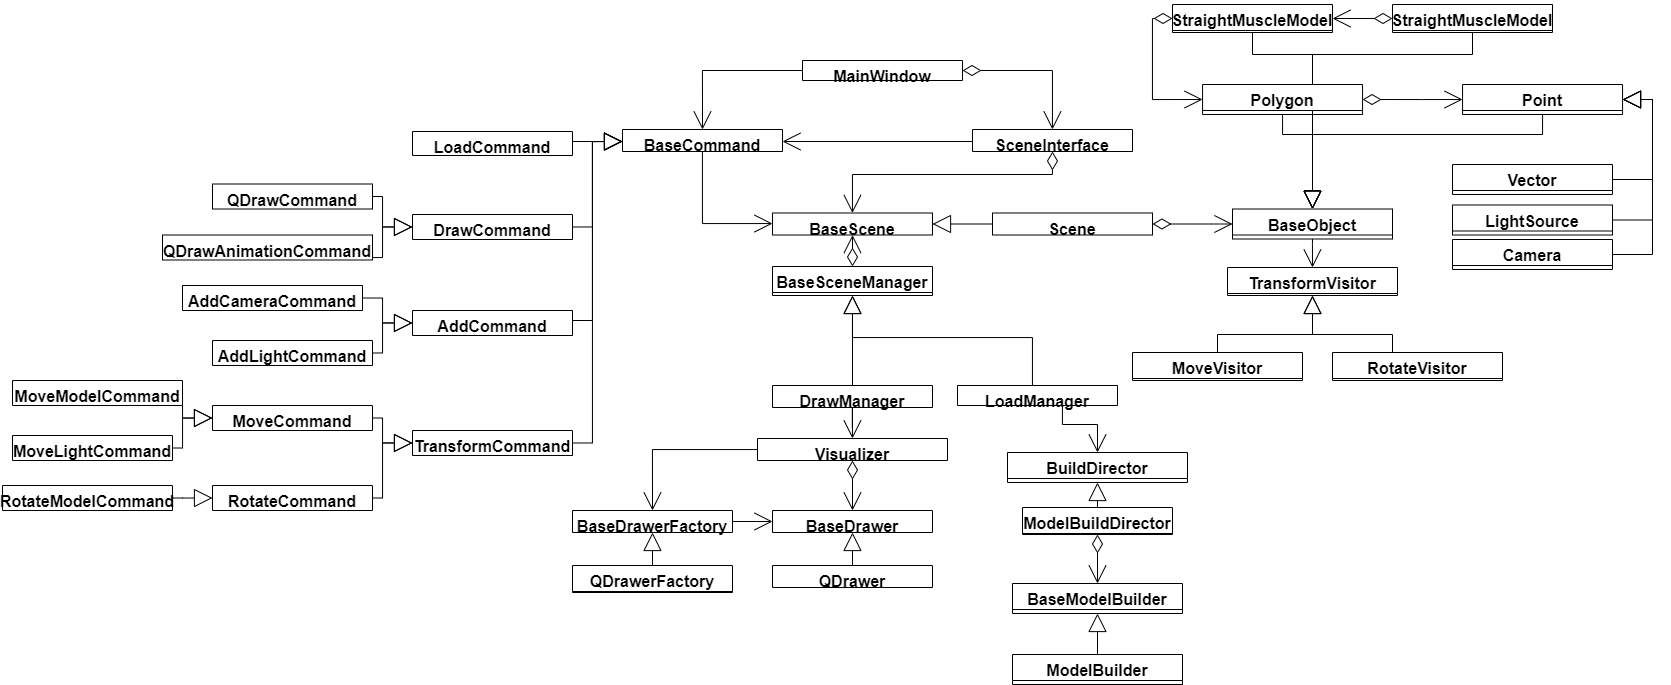
\includegraphics[height=0.35\paperheight, angle=90]{images/scheme}
	\caption{Диаграмма классов}
	\label{fig:scheme}
\end{figure}


\section{Листинг кода}
В листинге \ref{code:zbuf} представлен код класса Z-буффера, который содержит метод \Code{process\_polygon(self, polygon, light)} на вход которого подаётся полигон и массив источников света, а он растеризует поданный треугольник, вызывает метод для вычисления интенсивности цвета полигона и заполняет экранный и z-буфер.
\begin{lstlisting}[caption= Класс Z-буффера, label=code:zbuf]
	class ZBuffer(object):
		def __init__(self, visualizer, width=900, height=900):
			self.width = width
			self.height = height
			self.visualizer = visualizer
			self._buf = [[-6000 for _ in range(width)] for __ in range(height)]
			
		def process_polygon(self, polygon, light):
			color = polygon.get_color(light)
			
			points = polygon.get_points()
			x = [floor(points[i].x) for i in range(3)]
			y = [floor(points[i].y) for i in range(3)]
			
			ymax = min(max(y), self.height)
			ymin = min(min(y), 0)
			
			x1 = x2 = 0
			z1 = z2 = 0
			for y_current in range(ymin, ymax+1):
				first_cycle = 1
				for n in range(3):
					n1 = 0 if n == 2 else n + 1
					if y_current >= max(y[n], y[n1]) or y_current < min(y[n], y[n1]):
						continue
					
					m = float(y[n] - y_current) / (y[n]-y[n1])
					if first_cycle == 0:
						x2 = x[n] + floor(m * (x[n1] - x[n]))
						z2 = points[n].z + m * (points[n1].z - points[n].z)
					else:
						x1 = x[n] + floor(m * (x[n1] - x[n]))
						z1 = points[n].z + m * (points[n1].z - points[n].z)
						
					first_cycle = 0
				
				if x2 < x1:
					x2, x1 = x1, x2
					z2, z1 = z1, z2
					
				x_max = min(x2, self.width)
				x_min = max(x1, 0)
				for x_current in range(x_min, x_max):
					m = float(x1 - x_current) / (x1 - x2)
					z_current = z1 + m * (z2 - z1)
					self.process_point(x_current, y_current, int(z_current), color)
		
		def process_point(self, x: int, y: int, z: int, color):
			if z > self._buf[x][y]:
				self._buf[x][y] = z
				self.visualizer.drawPoint(x, y, color)
\end{lstlisting}
В листинге \ref{code:color} представлен метод вычисления интенсивности цвета полигона по формуле Ламберта. 
\begin{lstlisting}[caption= Метод рассчёта интенсивности цвета полигона, label=code:color]
	def get_color(self, lights):
		x, y, z = 0, 0, 0
		for p in self.get_points():
			xt, yt, zt = p.get_position()
			x += xt
			y += yt
			z += zt
		
		centroid = Point(x / 3, y / 3, z / 3)
		normal = self.get_normal().normalize()
		
		intensity = 0.4
		for light in lights:
			v = Vector().from_points(light, centroid).normalize()
			cos = max(v.scalar_multiplication(normal), 0)
			intensity += light.intensity * cos
			
		rgb = list(QColor(self.color).getRgbF())
		
		rgb[0] *= intensity
		rgb[1] *= intensity
		rgb[2] *= intensity
		
		return QColor().fromRgbF(rgb[0], rgb[1], rgb[2])
\end{lstlisting}

В листинге \ref{code:ellipse} представлен код класса эллипсоида, в котором в методе \Code{\_\_init\_\_(self)} определяются координаты вершин исходного куба, а в методе \Code{rec\_subdivide(self, d)} производится рекурсивное разбиение его полигонов.
\begin{lstlisting}[caption= Класс эллипсоида, label=code:ellipse]
	class Ellipsoid(object):
		def __init__(self):
			x = 1
			z = 1
			y = 1
			
			self.vertex_list = [
			[-x, -y, -z], [x, -y, -z], [x, -y, z], [-x, -y, z],
			[-x, y, -z], [x, y, -z], [x, y, z], [-x, y, z]
			]
			
			self.triangle_list = [
			[0,2,1], [0,3,2], [1,5,0], [5,4,0], [0,4,7], [7,3,0],
			[6,5,1], [1,2,6], [7,2,3], [7,6,2], [4,5,6], [6,7,4]
			]
			
			self.result_ind = []
			self.result_vertexes = []
		
		@staticmethod
		def normalize(v):
			d = sqrt(v[0] * v[0] + v[1] * v[1] + v[2] * v[2])
			if d == 0.0:
				print("zero division")
			v[0] /= d
			v[1] /= d
			v[2] /= d
		
		def start_division(self, d):
			self.result_ind = []
			self.result_vertexes = []
			for i in range(12):
				self.rec_subdivide( self.vertex_list[self.triangle_list[i][0]],
					self.vertex_list[self.triangle_list[i][1]],
					self.vertex_list[self.triangle_list[i][2]], d)
			
			for vertex in self.result_vertexes:
				self.normalize(vertex)
		
		def rec_subdivide(self, v1, v2, v3, d):
			v12 = [0, 0, 0]
			v23 = [0, 0, 0]
			v31 = [0, 0, 0]
			
			if d == 0:
				if v1 not in self.result_vertexes:
					self.result_vertexes.append(v1)
				if v2 not in self.result_vertexes:
					self.result_vertexes.append(v2)
				if v3 not in self.result_vertexes:
					self.result_vertexes.append(v3)
				t = [0, 0, 0]
				t[0] = self.result_vertexes.index(v1)
				t[1] = self.result_vertexes.index(v2)
				t[2] = self.result_vertexes.index(v3)
				
				self.result_ind.append(t)
				return
		
			for i in range(3):
				v12[i] = (v1[i] + v2[i]) / 2
				v23[i] = (v2[i] + v3[i]) / 2
				v31[i] = (v3[i] + v1[i]) / 2
			
			self.rec_subdivide(v1, v12, v31, d - 1)
			self.rec_subdivide(v2, v23, v12, d - 1)
			self.rec_subdivide(v3, v31, v23, d - 1)
			self.rec_subdivide(v12, v23, v31, d - 1)
		
		def reshape(self, x, y, z):
			for vertex in self.result_vertexes:
				vertex[0] *= x
				vertex[1] *= y
				vertex[2] *= z
			
		def polygonise(self, center_x=0, center_y=0, center_z=0):
			polygons = []
			for triangle in self.result_ind:
				p1 = Point(self.result_vertexes[triangle[0]][0] + center_x, self.result_vertexes[triangle[0]][1] + center_y, self.result_vertexes[triangle[0]][2] + center_z)
				p2 = Point(self.result_vertexes[triangle[1]][0] + center_x, self.result_vertexes[triangle[1]][1] + center_y, self.result_vertexes[triangle[1]][2] + center_z)
				p3 = Point(self.result_vertexes[triangle[2]][0] + center_x, self.result_vertexes[triangle[2]][1] + center_y, self.result_vertexes[triangle[2]][2] + center_z)
				polygons.append(Polygon(p1, p2, p3))
			return polygons
\end{lstlisting}

В листинге \ref{code:morph} представлен код класса Morph, который содержит в себе методы, необходимые для вычисления промежуточных мешей, а именно метод установления между начальными и результирующими полигонами \Code{straight\_map(self)} и метод \Code{calculate\_paths(self)}, рассчитывающий путь, который необходимо преодолеть каждой вершине каждого полигона.
\begin{lstlisting}[caption= Класс морфинга, label=code:morph]
	class Morph(object):
		def __init__(self, begin, end, frames=30):
			self.begin = begin
			self.end = end
			self.paths = []
			self.pairs = []
			
			self.frames = frames
			
			self.straight_map()
			self.calculate_paths()
			
		def straight_map(self):
			number = len(self.begin)
			self.pairs = [[i, i, 0] for i in range(number)]
			return self.pairs
		
		def calculate_paths(self):			
			for pair in self.pairs:
				p1 = self.begin[pair[0]].get_points()
				p2 = self.end[pair[1]].get_points()
				v3 = []
				for i in range(3):
					v = Vector()
					v.from_points(p1[i], p2[i])
					v3.append(v)
				
				self.paths.append(v3)
			
			return self.paths
		
		def get_frame(self, frame_number):
			number = len(self.begin)
			result = []
			
			for i in range(number):
				points = self.begin[self.pairs[i][0]].get_points()
				for p in range(3):
					points[p] = points[p] + \ self.paths[self.pairs[i][0]][p]. \ number_multiplication(frame_number) / self.frames
				result.append(Polygon(points[0], points[1], points[2], self.begin[self.pairs[i][0]].color))
			
			return result
\end{lstlisting}

\section{Интерфейс программы}
На рисунке \ref{fig:wholeinterface} представлен интерфейс программы.
\begin{figure}[H]
	\centering
	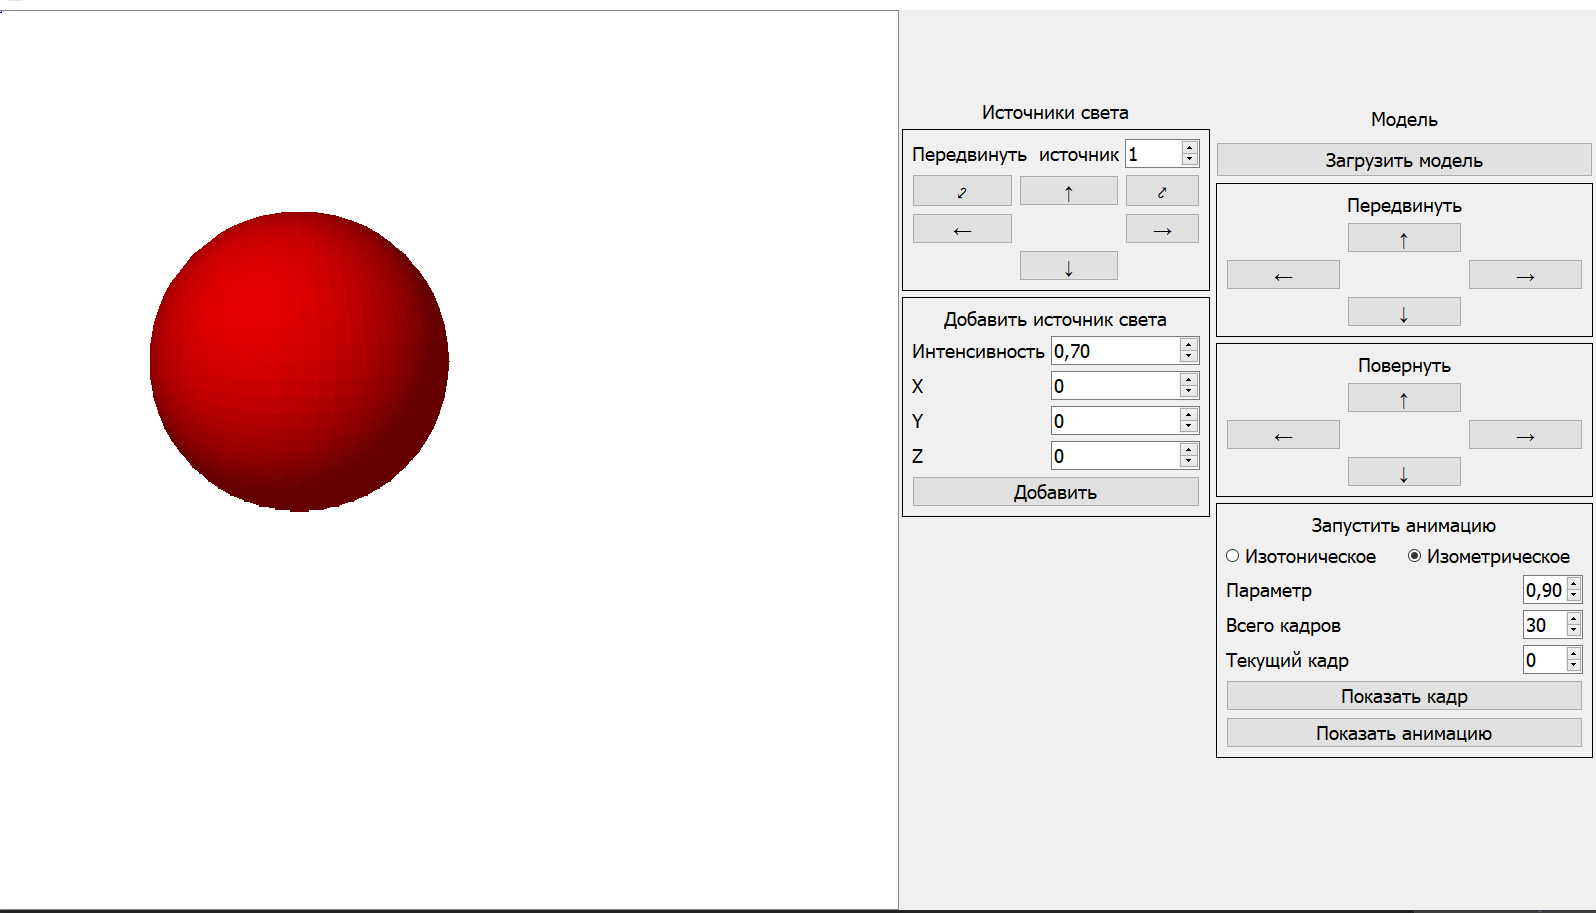
\includegraphics[width=0.9\linewidth]{images/whole_interface}
	\caption{Интерфейс программы}
	\label{fig:wholeinterface}
\end{figure}
Интерфейс включает в себя блок взаимодействия с источниками свет и блок взаимодействия с моделью. Первый, представленный на рисунке \ref{fig:lights}, предоставляет возможности:
\begin{itemize}
	\item передвинуть источник света в одном из 3 направлений;
	\item добавить новый источник света, задав его интенсивность и координаты.
\end{itemize}
\begin{figure}[H]
	\centering
	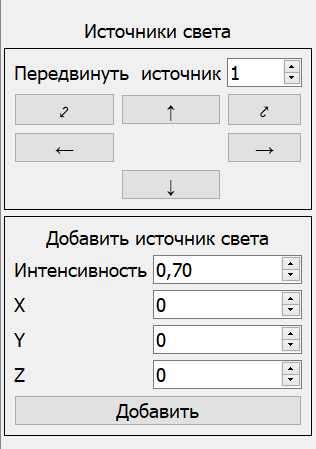
\includegraphics[width=0.4\linewidth]{images/lights}
	\caption{Блок взаимодействия с источниками света}
	\label{fig:lights}
\end{figure}

Второй блок, представленный на рисунке \ref{fig:models}, содержит поля, отвечающие за:
\begin{itemize}
	\item загрузку модели;
	\item перемещение и поворот модели;
	\item выбор типа сокращения -- изометрическое или изотоническое сокращение;
	\item выбор количества кадров анимации;
	\item отображение анимации и отдельных промежуточных кадров.
\end{itemize}
\begin{figure}[H]
	\centering
	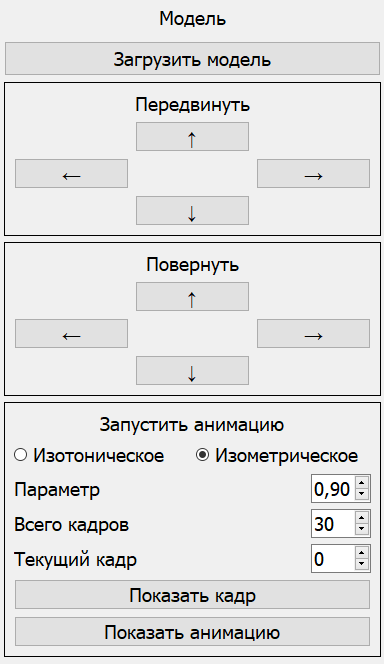
\includegraphics[width=0.4\linewidth]{images/models}
	\caption{Блок взаимодействия с моделями}
	\label{fig:models}
\end{figure}



\section{Вывод}
\label{sec:conc_impl}
В данном разделе были представлены средства, используемые для реализации выбранных алгоритмов, приведены листинги основных классов и функций. Также был рассмотрен реализованный интерфейс программы, модули и диаграмма классов.

%%%% mode: latex
%%%% TeX-master: "rpz"
%%%% End:
                                                                                                                                                 
%\chapter{Исследовательский раздел}
\label{cha:research}
В данном разделе будет проведено исследование реализованной программы.
\paragraph{Цель эксперимента} -- оценка времени выполнения алгоритмов в зависимости от количества полигонов.
\paragraph{Постановка эксперимента} -- эксперимент проводился на компьютере со следующими параметрами Intel(R) Core(TM) i5-8250, 8гб оперативной памяти, операционная система Windows 10. 
\par Количество полигонов изменялось за счёт увеличения числа рекурсивных повторений функции разбиения, так что их число можно посчитать по формуле
\begin{equation}
	p=12*4^n
\end{equation} 
где p -- число полигонов, n -- глубина рекурсии.
\par Для каждого n эксперимент проводился 5 раз, измерялось время для отрисовки 1 кадра, после чего результат усреднялся:
\begin{itemize}
	\item n=1, 48 полигонов, затраченное время 0,2с;
	\item n=2, 192 полигонов, затраченное время 0,24с;
	\item n=3, 768 полигонов, затраченное время 0,29с;
	\item n=4, 3072 полигонов, затраченное время 0,42с;
	\item n=5, 12288 полигонов, затраченное время 0,94с.
\end{itemize}
На рисунке \ref{fig:research} представлен график с результатами проведённого исследования.
\begin{figure}[H]
	\centering
	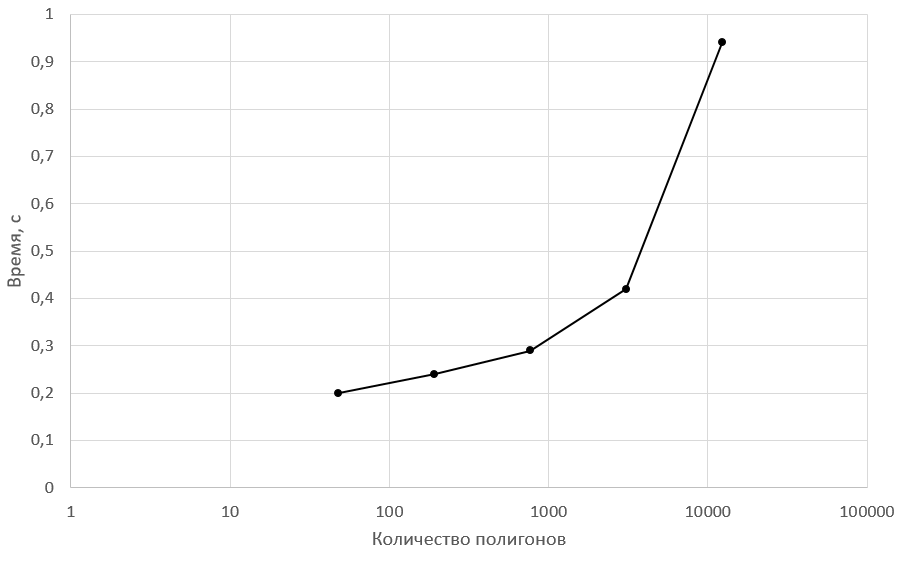
\includegraphics[width=0.7\linewidth]{images/research}
	\caption{График зависимости времени отрисовки одного кадра от количества полигонов}
	\label{fig:research}
\end{figure}

\paragraph{Вывод} из представленных результатов видно, что рост числа полигонов в 4 раза незначительно увеличивает время обработки модели, однако при увеличении глубины рекурсии с 4 до 5 затрачиваемое время растёт более чем в 2 раза, в то время как реалистичность изображения изменяется не сильно.


\backmatter %% Здесь заканчивается нумерованная часть документа и начинаются ссылки и
            
%\Conclusion % заключение к отчёту

%% заключение


% % Список литературы при помощи BibTeX
% Юзать так:
%
% pdflatex rpz
% bibtex rpz
% pdflatex rpz

\bibliographystyle{ugost2008}
\bibliography{rpz}

%%% Local Variables: 
%%% mode: latex
%%% TeX-master: "rpz"
%%% End: 


%
%\appendix   % Тут идут приложения
%
%\chapter{Реализация и тестирование}

%
%\include{91-appendix2}

\end{document}

%%% Local Variables:
%%% mode: latex
%%% TeX-master: t
%%% End:
